\documentclass[12pt]{article}
\usepackage[utf8]{inputenc}
\usepackage{mathtools}
\usepackage{graphicx}
\usepackage{subfig}
\usepackage{float}
\usepackage[export]{adjustbox}
\usepackage{amsmath}
\usepackage{listings}
\usepackage{color}

\graphicspath{{./report/}}

\definecolor{codegreen}{rgb}{0,0.6,0}
\definecolor{codegray}{rgb}{0.5,0.5,0.5}
\definecolor{codepurple}{rgb}{0.58,0,0.82}
\definecolor{backcolour}{rgb}{0.95,0.95,0.92}
 
\lstdefinestyle{mystyle}{
    backgroundcolor=\color{backcolour},   
    commentstyle=\color{codegreen},
    keywordstyle=\color{magenta},
    numberstyle=\tiny\color{codegray},
    stringstyle=\color{codepurple},
    basicstyle=\scriptsize,
    breakatwhitespace=false,         
    breaklines=true,                 
    captionpos=b,                    
    keepspaces=true,                 
    numbers=left,                    
    numbersep=5pt,                  
    showspaces=false,                
    showstringspaces=false,
    showtabs=false,                  
    tabsize=2
}
\lstset{style=mystyle}
\begin{document}
\title{CSC411 Project2}
\author{Yifei Ai}
\date{}
\maketitle
% ------------------------- Part 1 -------------------------
\section*{Part 1}
The dataset is a dictionary consisting of 9 training sets which are just number 0 to 9 and 9 test sets. Each training set is a matrix with $M\times 784$ which M represents the number of handwritten digit images in the dataset and each row is an array of size $1\times 784$ is the flatten array of handwritten digit image, which originally is $28\times 28$.

I randomly pick 10 images for each number, they all looks pretty good. At least I believe they are classified to the correct number.
\begin{figure}[h]
    \subfloat{{\includegraphics[width=0.2\textwidth]{report/train0.png}}}
    \subfloat{{\includegraphics[width=0.2\textwidth]{report/train1.png}}}
    \subfloat{{\includegraphics[width=0.2\textwidth]{report/train2.png}}}
    \subfloat{{\includegraphics[width=0.2\textwidth]{report/train3.png}}}
    \subfloat{{\includegraphics[width=0.2\textwidth]{report/train4.png}}}
    \caption{Digits Image 0 to 4}
\end{figure}
\begin{figure}[h]
    \subfloat{{\includegraphics[width=0.2\textwidth]{report/train5.png}}}
    \subfloat{{\includegraphics[width=0.2\textwidth]{report/train6.png}}}
    \subfloat{{\includegraphics[width=0.2\textwidth]{report/train7.png}}}
    \subfloat{{\includegraphics[width=0.2\textwidth]{report/train8.png}}}
    \subfloat{{\includegraphics[width=0.2\textwidth]{report/train9.png}}}
    \caption{Digits Image 0 to 5}
\end{figure}
% TODO: Include the image
% ------------------------- Part 2 -------------------------
\section*{Part 2}
Notice to make it convinient, I simply assume we already append the bias vector to Weight matrix
\begin{lstlisting}[language=Python]
    def layer_computation(x, W, b, act_func=lambda x: x):
        L = np.dot(W.T, x) + b
      	output = softmax(L)
      	return L, output

    def batch_layer_computation(X, W):
        """ X is an input matrix with size NxM, N is the number of input units, M is
        the number of training cases. W is a weight matrix already append bias vector 
        with size (N+1)xL, L is the number of output layers. Notice we need extra 
        one row for bias, so we should append another row vector [1, 1, 1, 1, ... ,1] 
        to X to do implement the function. """
        one_array = np.ones(X.shape[1])
        X = np.vstack((X, one_array))
        L1 = np.dot(W.T, X)
        Y = softmax(L1)
        return Y
\end{lstlisting}

% ------------------------- Part 3 -------------------------
\section*{Part 3}
Suppose X is a matrix with size $N\times M$, where N is the number of input layer, M is the number of training cases. Let W be a matrix be $N\times L$ where L is the number of units in hidden layer. Here L is 10. The output matrix Y has size of $L\times M$
\begin{align}
    % \frac{\partial \mathcal{L}_{CE}}{\partial y_k} &= \frac{-t_k}{y_k}\\
    % \mathcal{L}_{CE}(y, t) &= -t^T(logy)\\
    %                        &= -\sum_{j=1}^K t_j logy_j\\
    %                        &= -\sum_{j=1}^K t_j log\frac{e^{o_j}}{\sum_i e^{o_i}}\\
    %                        &= -\sum_{j=1}^K t_j (loge^{o_j} - log\sum_i e^{o_i})\\
    %                        &= -\sum_{j=1}^K t_j (o_j - log\sum_i e^{o_i})\\
    % \frac{\partial \mathcal{L}_{CE}}{\partial o_k} 
    % &= -t_k + \frac{e^{o_k}}{\sum_i e^{o_i}}\sum_{j=1}^K t_j && \text{Notice $\sum_{j=1}^K t_j = 1$}\\
    % &= -t_k + \frac{e^{o_k}}{\sum_i e^{o_i}}\\
    % &= -t_k + y_k\\
    % &= y_k - t_k
    y_j^{(i)} &= \frac{e^{o_j^{(i)}}}{\sum_k e^{o_k^{(i)}}}\\
    o_k^{(i)} &= \sum_{p=1}^{N}w_{pk}x_p^{(i)}+b_k\\
    \mathcal{L}_{CE} 
    &= \sum_{i=1}^M \sum_{j=0}^{L-1} -t_j^{(i)}logy_j^{(I)}\\
    &= \sum_{i=1}^M \sum_{j=0}^{L-1} -t_j^{(i)}[o_j^{(i)}-log(\sum_{k=0}^{L-1} e^{o_k^{(i)}})]\\
    &= \sum_{i=1}^M \sum_{j=0}^{L-1} -t_j^{(i)}[\sum_{p=1}^{N}w_{pj}x_p^{(i)}+b_j - log\sum_k (e^{\sum_{p=1}^{N}w_{pk}x_p^{(i)}+b_k})]\\
    \frac{\partial \mathcal{L}_{CE}}{\partial w_{sm}}
    &= \sum_{i=1}^M [(-t_m^{(i)} + \frac{e^{\sum_{s=1}^{N}w_{sm}x_s^{(i)}+b_m}}{\sum_k (e^{\sum_{p=1}^{N}w_{pk}x_p^{(i)}+b_k})}\sum_{j=0}^{L-1} t_j^{(i)})\,\,x_s^{(i)}]\\ \text{Notice $\sum_{j=1}^{L-1} t_j = 1$}\\
    &= \sum_{i=1}^M [(-t_m^{(i)} + \frac{e^{o_m^{(i)}}}{\sum_k e^{o_k^{(i)}}})x_s^{(i)}]\\
    &= \sum_{i=1}^M [(-t_m^{(i)} + y_m^{(i)})x_s^{(i)}]
\end{align}
Therefore, we get the derivative of weight is:
\[
    \frac{\partial \mathcal{L}_{CE}}{\partial W} = X(Y-T)^T
\]
To approximate the gradient, I use the following code:
\begin{lstlisting}[language=Python]
    def approx_CE_dWeight_single(X, W, T, p, q, t):
        """Approximate the derivative of single entry in Jacobian matrix"""
        new_weight = W.copy()
        new_weight[p][q] += t
        Y = batch_layer_computation(X, W)
        Y_h = batch_layer_computation(X, new_weight)
        df = part3_cross_entropy(Y_h, T) - part3_cross_entropy(Y, T)
        df = np.true_divide(df, t)
        return df

    def approx_CE_dWeight(X, W, T, t=1e-4):
        size = W.shape
        df_matrix = np.empty(size, dtype=np.float64)
        for i in range(size[0]):
            for j in range(size[1]):
                df_matrix[i][j] = approx_CE_dWeight_single(X, W, T, i, j, t)
        return df_matrix
\end{lstlisting}
I wrote some test case to test the function. Notice here W already append the bias vectors.
\begin{lstlisting}
In [130]: X
Out[130]: 
array([[1, 5],
       [2, 4]])

In [131]: W
Out[131]: 
array([[3., 4., 7.],
       [2., 5., 9.],
       [3., 2., 6.]])

In [143]: Y = ast2.batch_layer_computation(X, W)

In [144]: Y
Out[144]: 
array([[7.58255810e-10, 7.09547416e-23],
       [3.05902227e-07, 6.30511676e-16],
       [9.99999693e-01, 1.00000000e+00]])

In [133]: T
Out[133]: 
array([[1, 0],
       [0, 1],
       [0, 0]])

In [134]: ast2.CE_dWeight(X, Y, T)
Out[134]: 
array([[-1.        , -4.99999969,  5.99999969],
       [-2.        , -3.99999939,  5.99999939],
       [-1.        , -0.99999969,  1.99999969]])


In [135]: ast2.approx_CE_dWeight(ast2.batch_layer_computation, X, W, T)
Out[135]: 
array([[-1.        , -4.99999969,  5.99999969],
       [-2.        , -3.99999939,  5.99999939],
       [-1.        , -0.99999969,  1.99999969]])

In [184]: X
Out[184]: 
array([[2, 8],
       [1, 9]])

In [185]: W
Out[185]: 
array([[1., 7., 2.],
       [0., 7., 5.],
       [6., 8., 4.]])

In [186]: Y = ast2.batch_layer_computation(X, W)

In [187]: Y
Out[187]: 
array([[7.58255957e-10, 8.40859712e-50],
       [9.99999887e-01, 1.00000000e+00],
       [1.12535162e-07, 1.18506486e-27]])

In [188]: ast2.CE_dWeight(X, Y, T)
Out[188]: 
array([[-2.00000000e+00,  1.99999977e+00,  2.25070324e-07],
       [-9.99999999e-01,  9.99999887e-01,  1.12535162e-07],
       [-9.99999999e-01,  9.99999887e-01,  1.12535162e-07]])

In [189]: ast2.approx_CE_dWeight(X, W, T)
Out[189]: 
array([[-2.00000000e+00,  1.99999977e+00,  2.25099939e-07],
       [-9.99999999e-01,  9.99999887e-01,  1.12549969e-07],
       [-9.99999999e-01,  9.99999887e-01,  1.12549969e-07]])
\end{lstlisting}

% ------------------------- Part 4 -------------------------
\section*{Part 4}
I just randomly initialize each weight between $-0.4$ to $0.4$. For bias, I just let them be zeros. Then I try different learning rate, seems like learning rate with $10^{-4}$ to $10^{-5}$ have best performance. Then I try to display the image of the weights. I find image of weights for learning rate $10^{-5}$ have many noise there, so it might be overfitting, even though performance for $10^{-5}$ is $2\%$ higher than performance for $10^{-4}$. So I just choose the value between them $5\times 10^{-5}$. We can see that this learning rate works better than 1e-4. The following is my graph.
\begin{figure}[H]
    \subfloat{{\includegraphics[width=0.5\textwidth]{report/part4_cost_1e-4.png}}}
    \qquad
    \subfloat{{\includegraphics[width=0.5\textwidth]{report/part4_perform_1e-4.png}}}
    \caption{Learning rate $1e-4$}
\end{figure}
\begin{figure}[H]
    \subfloat{{\includegraphics[width=0.5\textwidth]{report/part4_cost_5e-05.png}}}
    \qquad
    \subfloat{{\includegraphics[width=0.5\textwidth]{report/part4_perform_5e-05.png}}}
    \caption{Learning rate $5e-5$}
\end{figure}
\begin{figure}[H]
    \subfloat{{\includegraphics[width=0.5\textwidth]{report/part4_cost_1e-05.png}}}
    \qquad
    \subfloat{{\includegraphics[width=0.5\textwidth]{report/part4_perform_1e-05.png}}}
    \caption{Learning rate $1e-5$}
\end{figure}
\begin{figure}[h]
    \subfloat{{\includegraphics[width=0.2\textwidth]{report/part4_wt_0lr_5e-05.png}}}
    \subfloat{{\includegraphics[width=0.2\textwidth]{report/part4_wt_1lr_5e-05.png}}}
    \subfloat{{\includegraphics[width=0.2\textwidth]{report/part4_wt_2lr_5e-05.png}}}
    \subfloat{{\includegraphics[width=0.2\textwidth]{report/part4_wt_3lr_5e-05.png}}}
    \subfloat{{\includegraphics[width=0.2\textwidth]{report/part4_wt_4lr_5e-05.png}}}
    \caption{Digits Image 0 to 4}
\end{figure}
\begin{figure}[h]
    \subfloat{{\includegraphics[width=0.2\textwidth]{report/part4_wt_5lr_5e-05.png}}}
    \subfloat{{\includegraphics[width=0.2\textwidth]{report/part4_wt_6lr_5e-05.png}}}
    \subfloat{{\includegraphics[width=0.2\textwidth]{report/part4_wt_7lr_5e-05.png}}}
    \subfloat{{\includegraphics[width=0.2\textwidth]{report/part4_wt_8lr_5e-05.png}}}
    \subfloat{{\includegraphics[width=0.2\textwidth]{report/part4_wt_9lr_5e-05.png}}}
    \caption{Digits Image 5 to 10}
\end{figure}

% ------------------------- Part 5 -------------------------
\section*{Part 5}
I just simply follow the algorithm, momentum is at line 29
\begin{lstlisting}[language=Python]
def gradient_descent(X, T, alpha=0.00001, EPS = 1e-5, max_iter = 300, mu = 0):
    """ X is the matrix of inputs, NxM, N is the number of input units, M is the 
    number of training cases. T is the matrix of results, size: LxM, L is the 
    number of output units """
    # Initialize a weight matrix
    size = [X.shape[0], T.shape[0]]
    print "Weight size is:" + str(size)
    W = initialize_weights(size)
    b = initialize_bias(T.shape[0])
    previous_W = W - 10*EPS
    previous_b = b - 10*EPS
    count = 0
    perform_dict = dict()

    summary = np.empty((6, 0), dtype=float)

    X_test, T_test, X_valid, T_valid = seperate_train_valid()

    p = 0
    
    while norm(W - previous_W)+norm(b - previous_b) > EPS and count < max_iter:
        previous_W = W.copy()
        b = b.copy()
        Y = batch_layer_computation(X, W, b)
        Y_test = batch_layer_computation(X_test, W, b)
        Y_valid = batch_layer_computation(X_valid, W, b)
        data = calculate_data(Y, T, Y_test, T_test, Y_valid, T_valid)
        summary = np.hstack((summary, data[:,None]))
        p = mu*p + alpha*CE_dWeight(X, Y, T)
        W = W - p
        b = b - alpha*CE_dBias(Y, T)
        print "Iter: " , count
        print "Weight: " , W
        print "Cost: " , part3_cross_entropy(Y, T)
        if count % (max_iter/5) == 0:
            print "Accuracy on test set: ", calculate_accuracy(Y, T)
            perform_dict[count] = (calculate_accuracy(Y, T), previous_W, previous_b)
        count += 1
    if mu == 0:
        np.save('tmp/part4_summary_data'+str(alpha), summary)
    else:
        np.save('tmp/part4_summary_data_momentum'+str(alpha), summary)
    return W, b, perform_dict
\end{lstlisting}
We can see that gradient descent with momentum converge much faster than the one without using momentum.
\begin{figure}[h]
    \subfloat{{\includegraphics[width=0.5\textwidth]{report/part5_cost_5e-05.png}}}
    \qquad
    \subfloat{{\includegraphics[width=0.5\textwidth]{report/part5_perform_5e-05.png}}}
    \caption{Learning rate $5\times 10^{-5}$}
\end{figure}

% ------------------------- Part 6 -------------------------
\section*{Part 6}
\subsection*{(a)}
\begin{figure}[H]
    \centering
    \includegraphics[scale=0.5]{./report/part6_parta2.png}
    \caption{Contour set with w1 and w2 around optimum}
\end{figure}

\subsection*{(b), (c)}
I tried several examples, these two demonstrate the feature of momentum
\begin{figure}[H]
    \subfloat{{\includegraphics[width=0.5\textwidth]{report/part6_partbc1.png}}}
    \qquad
    \subfloat{{\includegraphics[width=0.5\textwidth]{report/part6_partbc2.png}}}
    \caption{trajectory for gradient descent with moment and without momentum}
\end{figure}

\subsection*{(d)}
The trajectory with momentum goes to the optimum faster, but would get around the optimum in a very small range compare with the trajectory without momentum. This is because we have momentum, that somehow remembers the direction of last update.

\subsection*{(e)}
We should choose the pixel in the center of the image. Our image is 28*28, so if we choose some variable on the edge then either the gradient descent on those 2 variables stop on first several steps or have a very slow trajectory. I think this is becuase it is on the edge, so since other entries in W is already close to optimum, so the variable on the edge doesn't really affect the result, in other word, it probably because the input is 0 corresponds to that entry is 0, so it doesn't really affect too much.

\begin{figure}[H]
    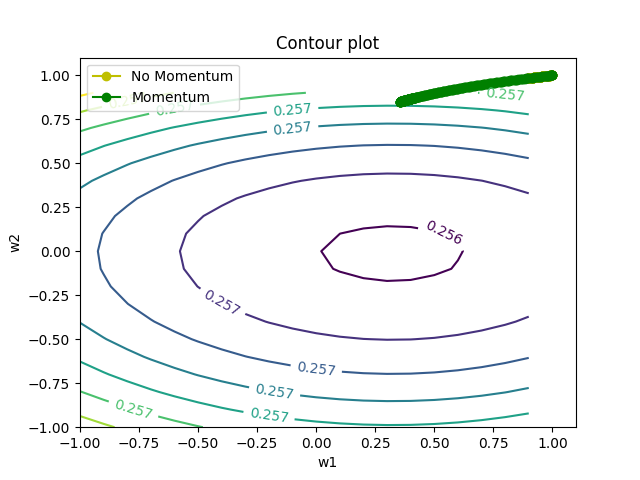
\includegraphics[width=\textwidth]{report/partbc_contour_bad.png}
    \caption{trajectory that doens't demonstrate the benefit of momentum}
\end{figure}

This is the w1, w2 from W[100][8] and W[200][8], if we check the train set $M['train8'][i][100]$ and $['train8'][i][200]$, most of them are 0. We can see that 2 trajectories are almost the same.

To get a nice example, I simply look for some entry in M['train8'][i] that is not 0, since 8 relatively has more entries be gray compare with other number in my opinion. Then I do the gradient descent to those 2 variables on the W.

% ------------------------- Part 7 -------------------------
\section*{Part 7}
Suppose we use back propagation, then, denote $T(N)$ as the complexity with N layers.
\begin{figure}[h]
    \centering
    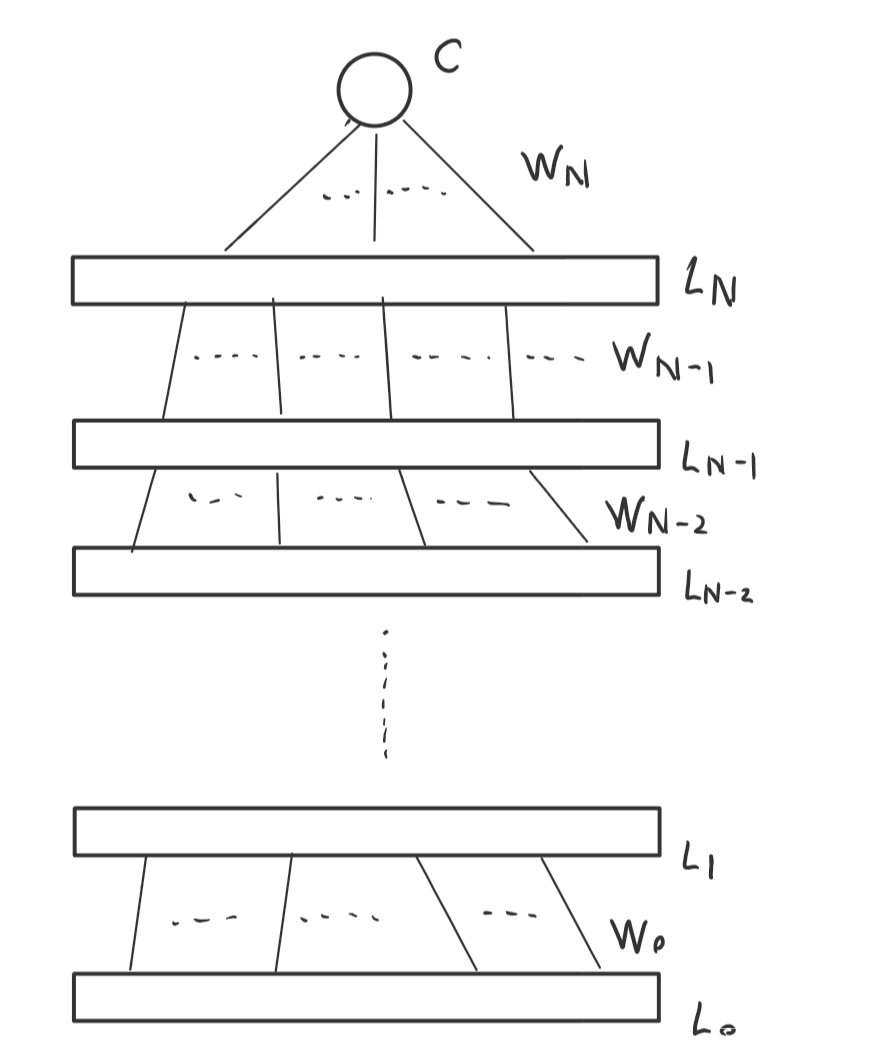
\includegraphics[scale=0.2]{report/part7_layer.jpg}
    \caption{Network with N+1 Layer}
\end{figure}
\subsection*{With Back Propagation}
Consider we have $N+1$ layers, now, if we need to calculate the gradients for all weights, then the first N layer we have calculate actually costs $T(N)$ by our assumption, then for the last layer, we need to know $\frac{\partial C}{\partial W_0}$. Since we use back propagation, we have $\frac{\partial C}{\partial L_2}$, thus we just need to calculate $\frac{\partial L_2}{\partial L_1}$ and $\frac{\partial L_1}{\partial W_0}$. So we will have
\[
    T(N+1) = T(N) + 2
\]
Which means complexity with back propagation is $O(N)$.
\subsection*{Without Back Propagation}
In this case, since we don't store any information, to calculate $\frac{\partial C}{\partial W_0}$, we need to do $\frac{\partial C}{\partial L_N}\frac{\partial L_N}{\partial L_{N-1}}\cdots \frac{\partial L_2}{\partial L_1}\frac{\partial L_1}{\partial W_0}$. So we will have
\[
    T(N+1) = T(N) + (N + 1)
\]
This means the complexity without back propagation is $O(N^2)$

% ------------------------- Part 8 -------------------------
\section*{Part 8}
I use a network with 32*32 or 64*64 input units, 6 output units, and one hidden layer. In that hidden layer, there are 12 hidden units, the activate function is ReLU. I tried both 32x32 and 64x64 to train the network. For 32x32 input, I set 64 hidden units, for 64x64 input, I set 32 hidden units. And I decide to use Adam optimizer. Since here the data is not very big, so I just set number of mini-batches as small as possible. Here are the final performance for each learning rate. The final performance on test set is around $75\%$ to $85\%$ if the learning rate is not too bad.
\begin{figure}[h]
    \subfloat[rate 1e-3]{{\includegraphics[width=0.28\textwidth]{report/part832_minibatch_loss1e-3.png}}}
    \qquad
    \subfloat[rate 1e-4]{{\includegraphics[width=0.28\textwidth]{report/part832_minibatch_loss1e-4.png}}}
    \qquad
    \subfloat[rate 1e-5]{{\includegraphics[width=0.28\textwidth]{report/part832_minibatch_loss1e-05.png}}}
    \caption{Resolution 32x32, learning curve with rate 0.01, 0.001, 0.0001}
\end{figure}
\begin{figure}[h]
    \subfloat[rate 1e-3]{{\includegraphics[width=0.28\textwidth]{report/part832_minibatch_performance1e-3.png}}}
    \qquad
    \subfloat[rate 1e-4]{{\includegraphics[width=0.28\textwidth]{report/part832_minibatch_performance1e-4.png}}}
    \qquad
    \subfloat[rate 1e-5]{{\includegraphics[width=0.28\textwidth]{report/part832_minibatch_performance1e-05.png}}}
    \caption{Resolution 32x32, learning curve with rate 0.01, 0.001, 0.0001}
\end{figure}
\begin{figure}[h]
    \subfloat[rate 1e-4]{{\includegraphics[width=0.5\textwidth]{report/part864_minibatch_loss1e-4.png}}}
    \qquad
    \subfloat[rate 1e-5]{{\includegraphics[width=0.5\textwidth]{report/part864_minibatch_loss1e-05.png}}}
    \caption{Resolution 64x64, learning curve with rate $10^{-4},10^{-5}$}
\end{figure}
\begin{figure}[H]
    \subfloat[rate 1e-4]{{\includegraphics[width=0.5\textwidth]{report/part864_minibatch_performance1e-4.png}}}
    \qquad
    \subfloat[rate 1e-5]{{\includegraphics[width=0.5\textwidth]{report/part864_minibatch_performance1e-05.png}}}
    \caption{Resolution 64x64, learning curve with rate $10^{-4},10^{-5}$}
\end{figure}

% ------------------------- Part 9 -------------------------
\section*{Part 9}
In this section, I actually change the number of mini-batches to 1. I also use the weight from the network for 64x64 size images cuz that somehow give more information. Then the strategy to find the most useful weights is the following. 
\begin{enumerate}
    \item Choose 2 actors, and look at the output nodes with respect to that actors
    \item For each actor, inspect the weights connected from hidden layer to that node
    \item Find the weight with hightest value, get the index of that weight, say it is k
    \item Inspect the $k^{th}$ node in the hidden layer, get the weight matrix from input layer to that node
    \item Convert that matrix to the image
\end{enumerate}
Here is my result, I choose gilpin and carell
\begin{figure}[H]
    \subfloat[gilpin]{{\includegraphics[width=0.45\textwidth]{report/part9_64_gilpin.png}}}
    \qquad
    \subfloat[carell]{{\includegraphics[width=0.45\textwidth]{report/part9_64_carell.png}}}
    \caption{Image of Weights}
\end{figure}

% ------------------------- Part 10 -------------------------
\section*{Part 10}
I construct a network whose input size matches the output from AlexNet.feature which is 256*6*6, I use 12 hidden units in the hidden layer, and the activate function is ReLU. I use Adam optimizer, with learning rate 1e-5, get $91.6\%$ performance on test set.
\end{document}